%%%%%%%%%%%%%%%%%%%%%%%%%%%%%%%%%%%%%%%%%%%%%%%%%%%%%%%%%%%%%%%%%%%%%
%% This is a (brief) model paper using the achemso class
%% The document class accepts keyval options, which should include
%% the target journal and optionally the manuscript type. 
%%%%%%%%%%%%%%%%%%%%%%%%%%%%%%%%%%%%%%%%%%%%%%%%%%%%%%%%%%%%%%%%%%%%%
\documentclass[journal=jacsat,manuscript=article]{achemso}

%%%%%%%%%%%%%%%%%%%%%%%%%%%%%%%%%%%%%%%%%%%%%%%%%%%%%%%%%%%%%%%%%%%%%
%% Place any additional packages needed here.  Only include packages
%% which are essential, to avoid problems later. Do NOT use any
%% packages which require e-TeX (for example etoolbox): the e-TeX
%% extensions are not currently available on the ACS conversion
%% servers.
%%%%%%%%%%%%%%%%%%%%%%%%%%%%%%%%%%%%%%%%%%%%%%%%%%%%%%%%%%%%%%%%%%%%%
\usepackage[version=3]{mhchem} % Formula subscripts using \ce{}

%%%%%%%%%%%%%%%%%%%%%%%%%%%%%%%%%%%%%%%%%%%%%%%%%%%%%%%%%%%%%%%%%%%%%
%% If issues arise when submitting your manuscript, you may want to
%% un-comment the next line.  This provides information on the
%% version of every file you have used.
%%%%%%%%%%%%%%%%%%%%%%%%%%%%%%%%%%%%%%%%%%%%%%%%%%%%%%%%%%%%%%%%%%%%%
%%\listfiles

%%%%%%%%%%%%%%%%%%%%%%%%%%%%%%%%%%%%%%%%%%%%%%%%%%%%%%%%%%%%%%%%%%%%%
%% Place any additional macros here.  Please use \newcommand* where
%% possible, and avoid layout-changing macros (which are not used
%% when typesetting).
%%%%%%%%%%%%%%%%%%%%%%%%%%%%%%%%%%%%%%%%%%%%%%%%%%%%%%%%%%%%%%%%%%%%%
%%\newcommand*\mycommand[1]{\texttt{\emph{#1}}}

\newcommand{\YE}[1]{\textcolor{blue}{#1}}

%%%%%%%%%%%%%%%%%%%%%%%%%%%%%%%%%%%%%%%%%%%%%%%%%%%%%%%%%%%%%%%%%%%%%
%% Meta-data block
%% ---------------
%% Each author should be given as a separate \author command.
%%
%% Corresponding authors should have an e-mail given after the author
%% name as an \email command. Phone and fax numbers can be given
%% using \phone and \fax, respectively; this information is optional.
%%
%% The affiliation of authors is given after the authors; each
%% \affiliation command applies to all preceding authors not already
%% assigned an affiliation.
%%
%% The affiliation takes an option argument for the short name.  This
%% will typically be something like "University of Somewhere".
%%
%% The \altaffiliation macro should be used for new address, etc.
%% On the other hand, \alsoaffiliation is used on a per author basis
%% when authors are associated with multiple institutions.
%%%%%%%%%%%%%%%%%%%%%%%%%%%%%%%%%%%%%%%%%%%%%%%%%%%%%%%%%%%%%%%%%%%%%
\author{Ye Ding}
\affiliation{ATOMBEAT Inc.}
\email{dingy01@dp.tech}
\author{Hang Zheng}
\affiliation{ATOMBEAT Inc.}
\author{Xi Chen}
\affiliation{ATOMBEAT Inc.}
\author{Dongxu Pan}
\affiliation{ATOMBEAT Inc.}
\author{Xinyan Wang}
\affiliation{ATOMBEAT Inc.}

%%%%%%%%%%%%%%%%%%%%%%%%%%%%%%%%%%%%%%%%%%%%%%%%%%%%%%%%%%%%%%%%%%%%%
%% The document title should be given as usual. Some journals require
%% a running title from the author: this should be supplied as an
%% optional argument to \title.
%%%%%%%%%%%%%%%%%%%%%%%%%%%%%%%%%%%%%%%%%%%%%%%%%%%%%%%%%%%%%%%%%%%%%
\title[An \textsf{achemso} demo]
  {Improving binding free energy predictions with Swap Monte Carlo for water sampling}

%%%%%%%%%%%%%%%%%%%%%%%%%%%%%%%%%%%%%%%%%%%%%%%%%%%%%%%%%%%%%%%%%%%%%
%% Some journals require a list of abbreviations or keywords to be
%% supplied. These should be set up here, and will be printed after
%% the title and author information, if needed.
%%%%%%%%%%%%%%%%%%%%%%%%%%%%%%%%%%%%%%%%%%%%%%%%%%%%%%%%%%%%%%%%%%%%%
\abbreviations{Free Energy Perturbation, Binding Free Energy, Monte Carlo, Water Sampling, Molecular Dynamics}
\keywords{American Chemical Society, \LaTeX}

%%%%%%%%%%%%%%%%%%%%%%%%%%%%%%%%%%%%%%%%%%%%%%%%%%%%%%%%%%%%%%%%%%%%%
%% The manuscript does not need to include \maketitle, which is
%% executed automatically.
%%%%%%%%%%%%%%%%%%%%%%%%%%%%%%%%%%%%%%%%%%%%%%%%%%%%%%%%%%%%%%%%%%%%%
\begin{document}

%%%%%%%%%%%%%%%%%%%%%%%%%%%%%%%%%%%%%%%%%%%%%%%%%%%%%%%%%%%%%%%%%%%%%
%% The "tocentry" environment can be used to create an entry for the
%% graphical table of contents. It is given here as some journals
%% require that it is printed as part of the abstract page. It will
%% be automatically moved as appropriate.
%%%%%%%%%%%%%%%%%%%%%%%%%%%%%%%%%%%%%%%%%%%%%%%%%%%%%%%%%%%%%%%%%%%%%
%\begin{tocentry}

%Some journals require a graphical entry for the Table of Contents.
%This should be laid out ``print ready'' so that the sizing of the
%text is correct.

%Inside the \texttt{tocentry} environment, the font used is Helvetica
%8\,pt, as required by \emph{Journal of the American Chemical
%Society}.

%The surrounding frame is 9\,cm by 3.5\,cm, which is the maximum
%permitted for  \emph{Journal of the American Chemical Society}
%graphical table of content entries. The box will not resize if the
%content is too big: instead it will overflow the edge of the box.

%This box and the associated title will always be printed on a
%separate page at the end of the document.

%\end{tocentry}

%%%%%%%%%%%%%%%%%%%%%%%%%%%%%%%%%%%%%%%%%%%%%%%%%%%%%%%%%%%%%%%%%%%%%
%% The abstract environment will automatically gobble the contents
%% if an abstract is not used by the target journal.
%%%%%%%%%%%%%%%%%%%%%%%%%%%%%%%%%%%%%%%%%%%%%%%%%%%%%%%%%%%%%%%%%%%%%
\begin{abstract}
Water molecules within and around the binding cavity can significantly influence the binding affinity of ligands. 
Proper sampling of these water molecules ensures that their contributions to the free energy landscape are accurately accounted for. 
In the pursuit of more accurate binding free energy calculations, we have developed a novel Swap Monte Carlo (SwapMC) method specifically designed for cavity water sampling. 
The SwapMC method aims to enhance the sampling efficiency by facilitating the movement of water molecules in and out of the protein cavity, thereby ensuring a comprehensive exploration of water distributions. 
By leveraging GPU power to perform Monte Carlo moves for water molecules in parallel across multiple sites, and integrating SwapMC with NPT simulations within the Uni-FEP framework, 
we have observed significant improvements in the accuracy of relative binding free energy calculations, all while maintaining computational efficiency. 
Our results demonstrate that SwapMC achieves performance comparable to Grand Canonical Monte Carlo (GCMC) methods in water-related test cases, offering a robust and efficient alternative for addressing the challenges associated with cavity water sampling in computational chemistry. 
%Furthermore, we have extended the SwapMC scheme to sample the distribution of ions in DNA/RNA simulations, 
%broadening the applicability of this method to a wider range of biomolecular systems and enhancing the accuracy of ion-related free energy calculations.
\end{abstract}

%%%%%%%%%%%%%%%%%%%%%%%%%%%%%%%%%%%%%%%%%%%%%%%%%%%%%%%%%%%%%%%%%%%%%
%% Start the main part of the manuscript here.
%%%%%%%%%%%%%%%%%%%%%%%%%%%%%%%%%%%%%%%%%%%%%%%%%%%%%%%%%%%%%%%%%%%%%
\section{Introduction}
%%\YE{TO be completed.}

\section{Method}
\subsection{Workflow of the Swap Monte Carlo}
SwapMC was designed to exchange water molecules in and out of the protein cavity during FEP calculations, Fig.~\ref{fgr:scheme} B.
The cavity region is defined as a spherical space centered at the geometric center of the ligand coordinates\cite{ben2021fast}, $R^{in}$ in Fig.~\ref{fgr:scheme}.
The radius is half the maximum intra-atomic distance within the ligands, plus an additional 0.3 nanometers for buffer.
All other areas of the simulation box are considered outside this spherical cavity and will be referred to as $R^{out}$ space hereafter, Fig.~\ref{fgr:scheme} A.
Thus, the SwapMC algorithm workflow consists of these steps:
\begin{enumerate}
  \item Randomly decide the exchange direction, ensuring an equal chance of moving water in or out of the cavity.
  \item A water molecule $i$ is chosen for deletion from the source region with the probability defined in Eq.~\ref{eq:selection_probability}. 
    Where $u_i$ represents the interaction energy of water molecule $i$ with other atoms in the simulation box. 
    $N_{src}$ denotes the number of exchangeable water molecules in the source region. A higher $u_i$ increases the likelihood of a molecule being selected.
  \begin{equation}\label{eq:selection_probability}
     p_i = \frac{e^{u_i}}{\sum^{N_{src}}_k{e^{u_k}}} \tag{1}    
  \end{equation}
  \item Uniform sampling the potential insertion sites over the destination region.
  \item The combination of the sampled sites with 60 orientations of water molecule results in 18,000 possible insertion conformations.
  \item Evaluate the interaction energy for each of the 18,000 water molecules in the simulated system, denoted as $u_j$.
  \item Sequentially iterate over these $u_j$ values, and calculate the acceptance ratio using $u_i$ and $u_j$, determine if the conformation is acceptable. If it is, terminate this iteration.
  \item Replace the deleted water positions by the accepted conformation coordinates and set this water molecule's velocity to zero.
\end{enumerate}

\begin{figure}
  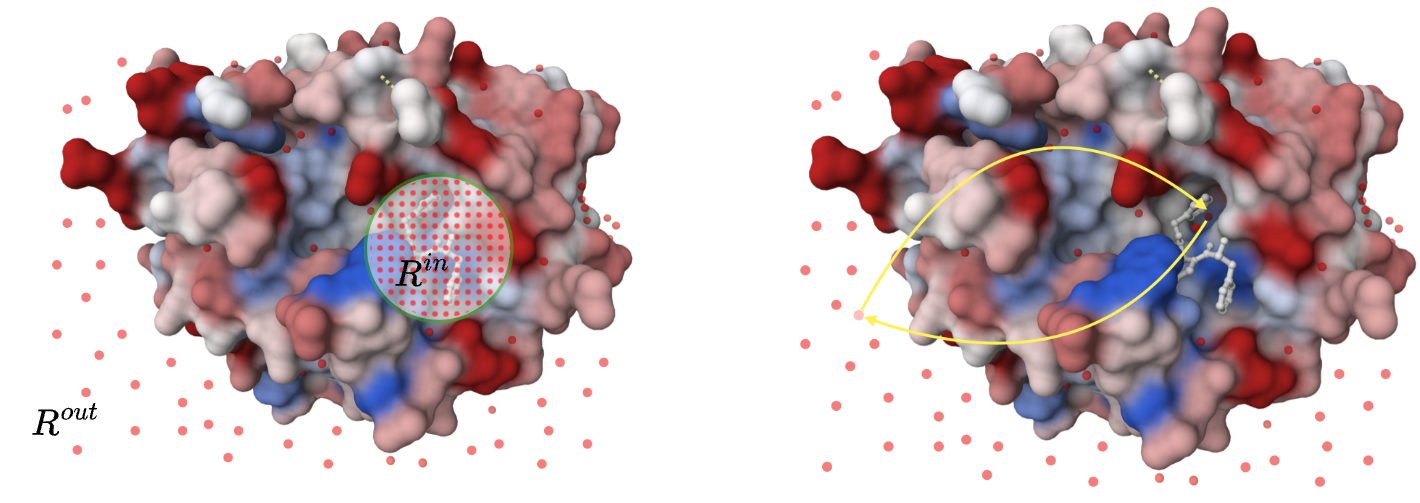
\includegraphics[width=0.9\textwidth]{figures/SwapMonteCarlo-scheme.png}
  \caption{Schematic Figure for Swap Monte Carlo (SwapMC) Method.
  The figure illustrates the process of moving water molecules in and out of the protein cavity during simulation.}
  \label{fgr:scheme}
\end{figure}

\subsection{Detailed Balance in Swap Monte Carlo}
In the Monte Carlo algorithm, the acceptance ratio between two states $S_i$ and $S_j$ must satisfy detailed balance:
\begin{equation}\label{eq:acceptance_ratio}
\frac{g_{S_i S_j} A_{S_i S_j}}{g_{S_j S_i} A_{S_j S_i}}=\frac{P_S_j}{P_S_i}  
\end{equation}


\section{Results}

\subsection{Water Density }


\subsection{}

\section{Discussion}






\section{Experimental}

\begin{table}
  \caption{An example table}
  \label{tbl:example}
  \begin{tabular}{ll}
    \hline
    Header one  & Header two  \\
    \hline
    Entry one   & Entry two   \\
    Entry three & Entry four  \\
    Entry five  & Entry five  \\
    Entry seven & Entry eight \\
    \hline
  \end{tabular}
\end{table}



\section{Extra information when writing JACS Communications}


%%%%%%%%%%%%%%%%%%%%%%%%%%%%%%%%%%%%%%%%%%%%%%%%%%%%%%%%%%%%%%%%%%%%%
%% The "Acknowledgement" section can be given in all manuscript
%% classes.  This should be given within the "acknowledgement"
%% environment, which will make the correct section or running title.
%%%%%%%%%%%%%%%%%%%%%%%%%%%%%%%%%%%%%%%%%%%%%%%%%%%%%%%%%%%%%%%%%%%%%
\begin{acknowledgement}

Please use ``The authors thank \ldots'' rather than ``The
authors would like to thank \ldots''.

The author thanks Mats Dahlgren for version one of \textsf{achemso},
and Donald Arseneau for the code taken from \textsf{cite} to move
citations after punctuation. Many users have provided feedback on the
class, which is reflected in all of the different demonstrations
shown in this document.

\end{acknowledgement}

%%%%%%%%%%%%%%%%%%%%%%%%%%%%%%%%%%%%%%%%%%%%%%%%%%%%%%%%%%%%%%%%%%%%%
%% The same is true for Supporting Information, which should use the
%% suppinfo environment.
%%%%%%%%%%%%%%%%%%%%%%%%%%%%%%%%%%%%%%%%%%%%%%%%%%%%%%%%%%%%%%%%%%%%%
\begin{suppinfo}

This will usually read something like: ``Experimental procedures and
characterization data for all new compounds. The class will
automatically add a sentence pointing to the information on-line:

\end{suppinfo}

%%%%%%%%%%%%%%%%%%%%%%%%%%%%%%%%%%%%%%%%%%%%%%%%%%%%%%%%%%%%%%%%%%%%%
%% The appropriate \bibliography command should be placed here.
%% Notice that the class file automatically sets \bibliographystyle
%% and also names the section correctly.
%%%%%%%%%%%%%%%%%%%%%%%%%%%%%%%%%%%%%%%%%%%%%%%%%%%%%%%%%%%%%%%%%%%%%
\bibliography{ref, common_ref}

\end{document}